\subsection{Plant Model in Simulink\textregistered}
\label{sec:plant}

\subsubsection{Motivation}
To test designed controllers, a representation of the plant to experiment on is needed.
Simulink\footnote{Simulink is a Registered Trademark of The MathWorks Inc.} was used to build a model of the plant, and apply controllers to.
The model is a \emph{simplified version} of how the plant is expected to behave.
The simplifications made and design decisions that were proceeded with are justified below.

\subsubsection{Modelled Components}

Components were simplified as how the many considered components will respond to changes of input are not known in detail.
Since the plant controls $P_{\text{net}}$, the SOFCs and the Turbine are important to simulate on the generation, and the electrolyser on the consumption side.

Tanks were modelled by means of a integrator, fed with net flow-rates for each chemical species.

The cryogenic air-still is kept running continuously as it reduces the size of the part required to make the same amount of material.
Another benefit is this negates the need to model the delay associated with priming the system before use.
Cryogenic stills take on the order of hours to reach the temperature required for operation, so continuous running makes sense from a energy conservation standpoint too.

\subsubsection{Assumptions}

Components were assumed to behave as first-order, linear with no delays.
There was also the assumption that there is no minimum utilisation for components, i.e. $0 \leq u \leq 1$ such that for example the electrolyser can drain any power between $0$ Watts and its maximum power, $P_{\text{max}}$.
For material flow-rate, it was assumed the ammonia used in the turbine and the SOFC scaled linearly with utilisation, and gas generation from the electrolyser also scaled linearly with utilisation.

\subsubsection{Simulink Model Structure and Initial Implementation}

Values for each block were left as variables to be determined by a supporting MATLAB script, with relevant data input from other sections of this investigation.
This allowed for rapid prototyping, and gave the ability to quickly try different values for controller gains to observe responses.
The model was subdivided into different components:
\begin{description}
\item[Global Plant]{ is a block that includes the plant and controller.
This is packaged in a convenient way as to apply different disturbances and observe performance.
A manual switch was added to move between real data and simulated disturbances.
All blocks below are inside the `Global Plant' block, modelled by Figure \ref{fig:plant}, which exists in the Testing Environment Figure \ref{fig:global}.}
\begin{description}
        \item[Grid Dynamics]{ in form of the `Swing Equation' was packaged to allow for adding more complicated coupling or measurement effects - yet this was not implemented. Grid Dynamics is modelled in Figure \ref{fig:grid}.}
        \item[Component Dynamics]{ encapsulates the different behaviours of each component, including the limits on control inputs, rise times, maximum power, material flow-rates and room to make component models more complex. Component dynamics are modelled in Figure \ref{fig:comp}.}
        \item[Controller]{ allows for controllers to be applied with multi-state feedback, with room to add complexity. In the diagrams below (Figure \ref{fig:ctrl}) the LQR with augmented state is implemented.}
        \item[Cryogenic Still]{ simulates basic, steady state behaviour of the cryogenic still, observed in Figure \ref{fig:cryo}.}
        \item[Tanks and Haber Column]{ simulates material volumes from flow-rates into a tank, and conversion of tank materials in the Haber Column. This system is modelled in Figure \ref{fig:tank}.}
\end{description}
\end{description}
The diagrams overleaf show the Simulink plant that was used with the this design study.

\begin{figure}[p]
\centering
        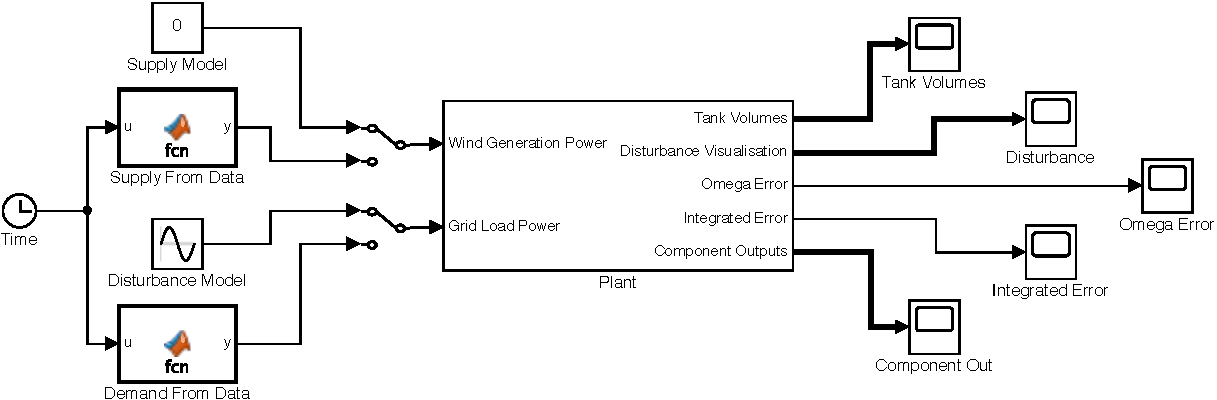
\includegraphics[scale=0.7]{images/plant/global.pdf}
        \caption{Plant in Testing Environment}
        \label{fig:global}
\end{figure}
\begin{figure}[p]
\centering
        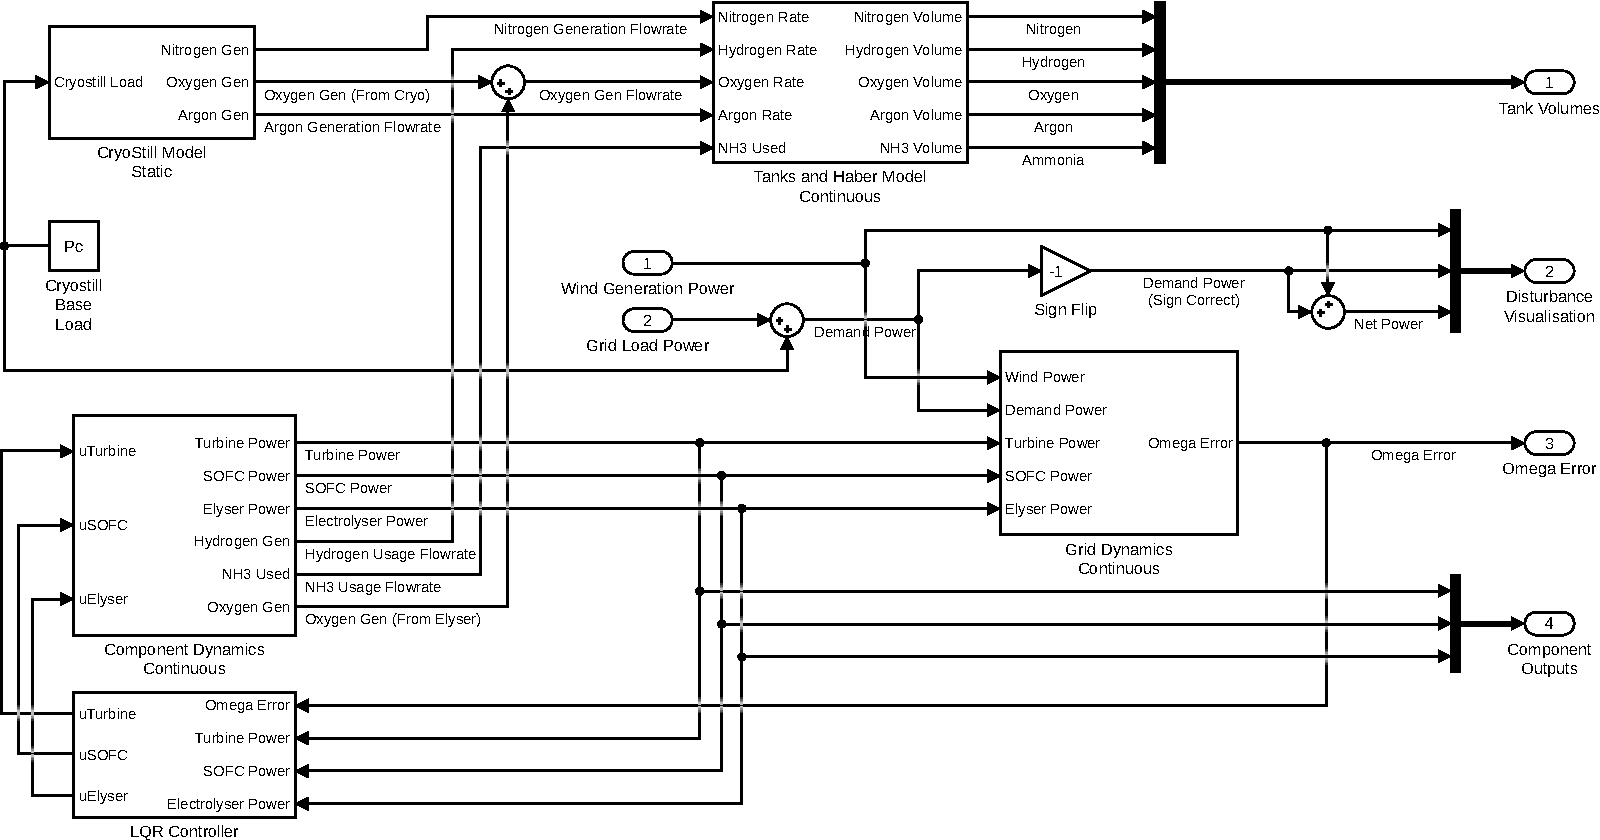
\includegraphics[scale=0.6]{images/plant2/plant.pdf}
    \caption{Plant with Controller Implemented}
        \label{fig:plant}
\end{figure}
\begin{figure}[p]
\centering
        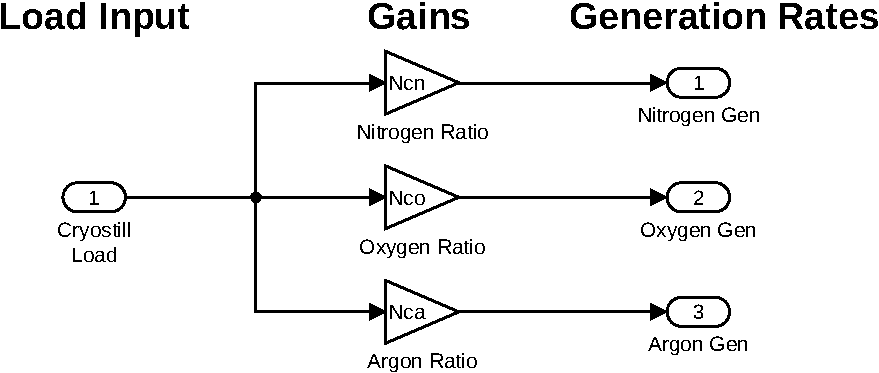
\includegraphics[scale=0.7]{images/plant2/cryo.pdf}
    \caption{Steady State Cryogenic Still Model}
        \label{fig:cryo}
\end{figure}
\begin{figure}[p]
\centering
        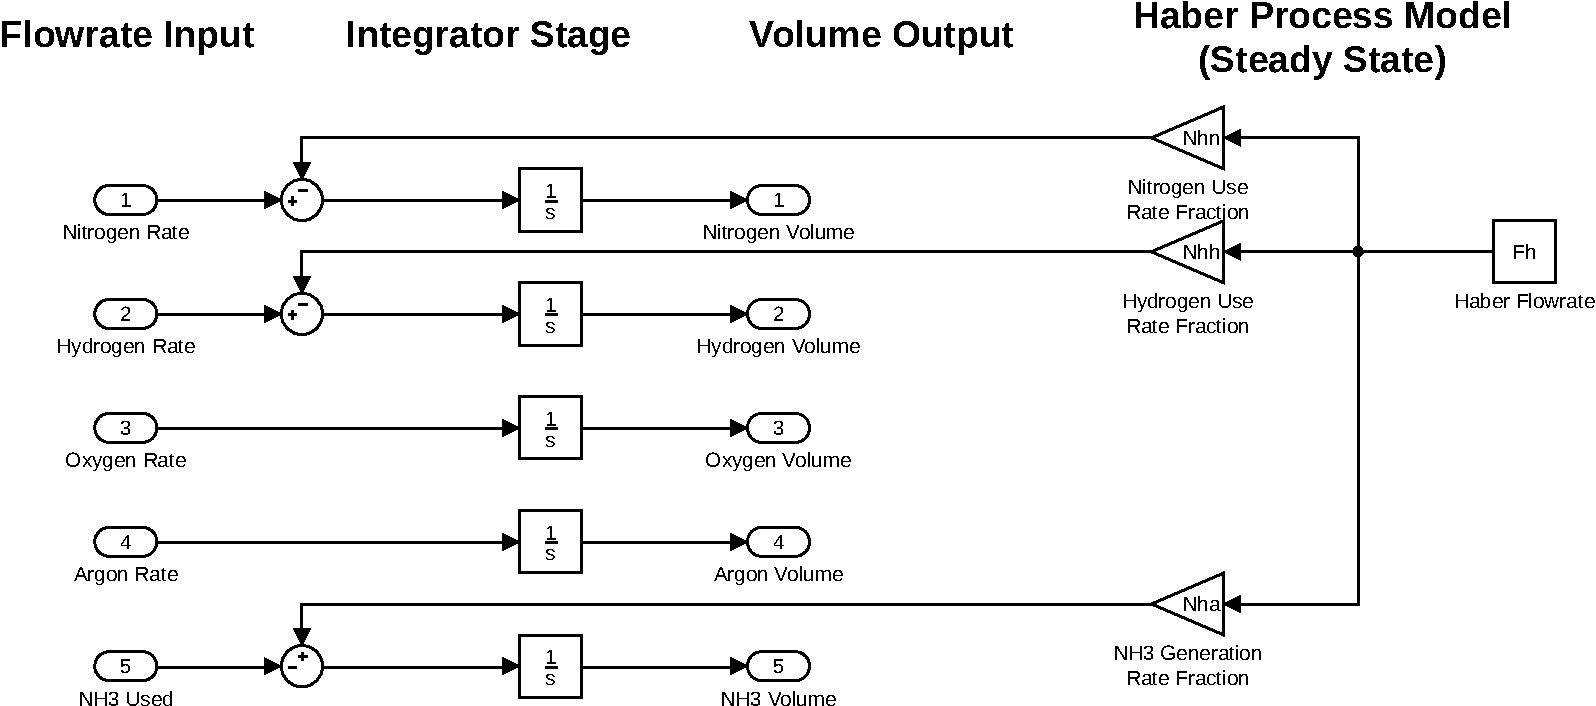
\includegraphics[scale=0.65]{images/plant2/tank.pdf}
    \caption{Tank and Steady State Haber Column Model}
        \label{fig:tank}
\end{figure}
\begin{figure}[p]
\centering
        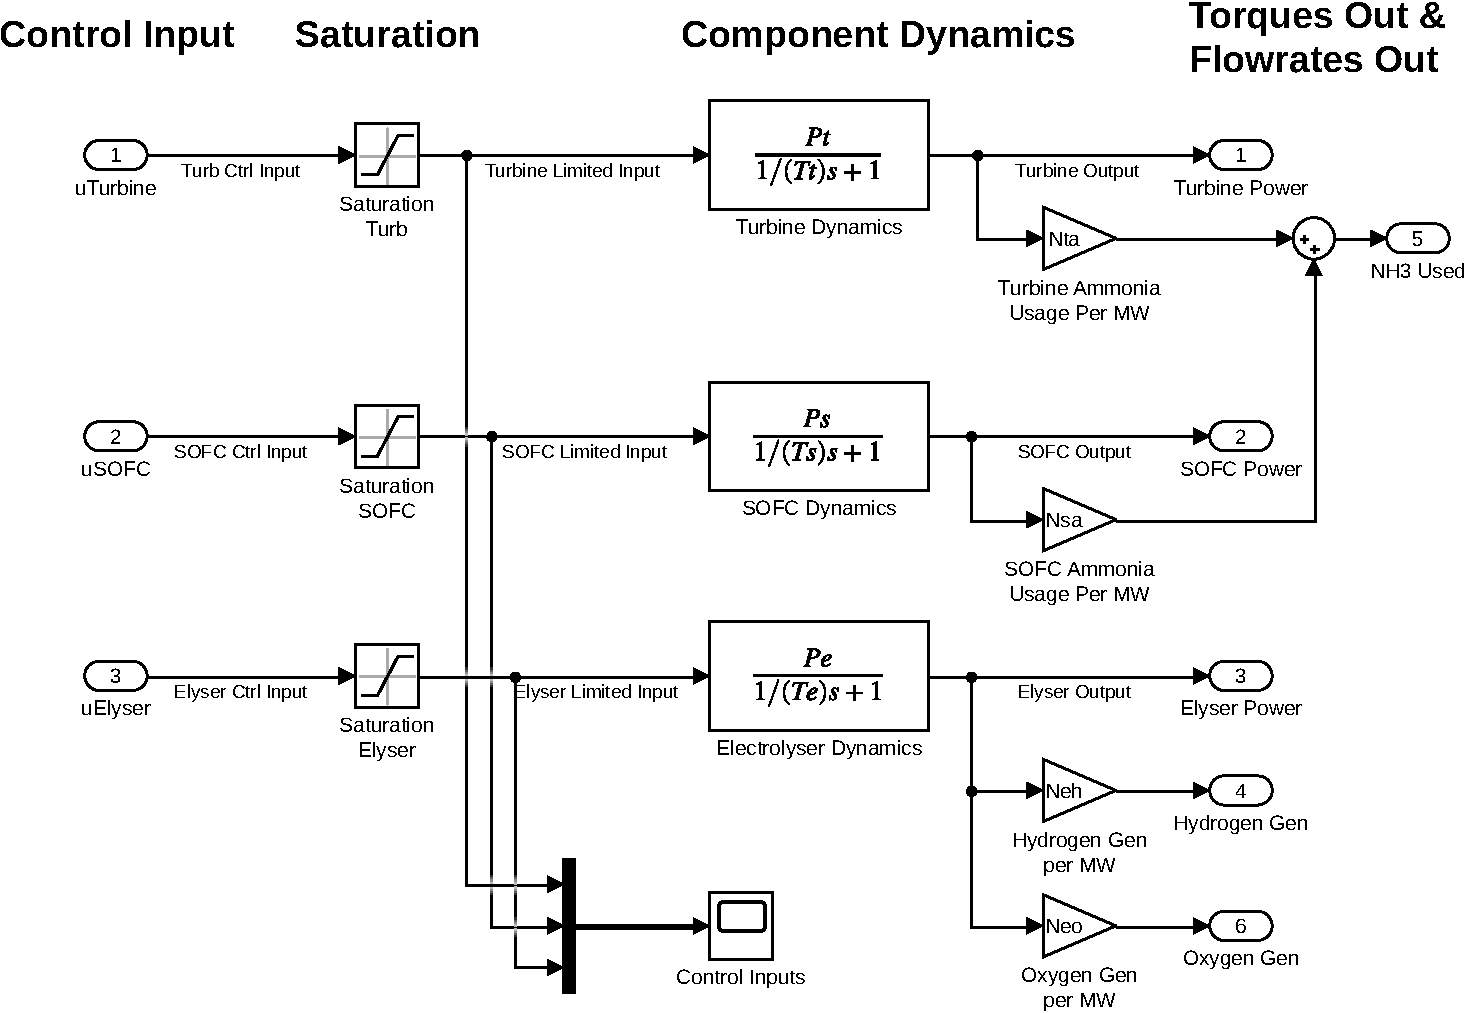
\includegraphics[scale=0.7]{images/plant2/comp.pdf}
    \caption{Component Dynamics (First Order Linear) with Saturation on Inputs}
        \label{fig:comp}
\end{figure}
\begin{figure}[p]
\centering
        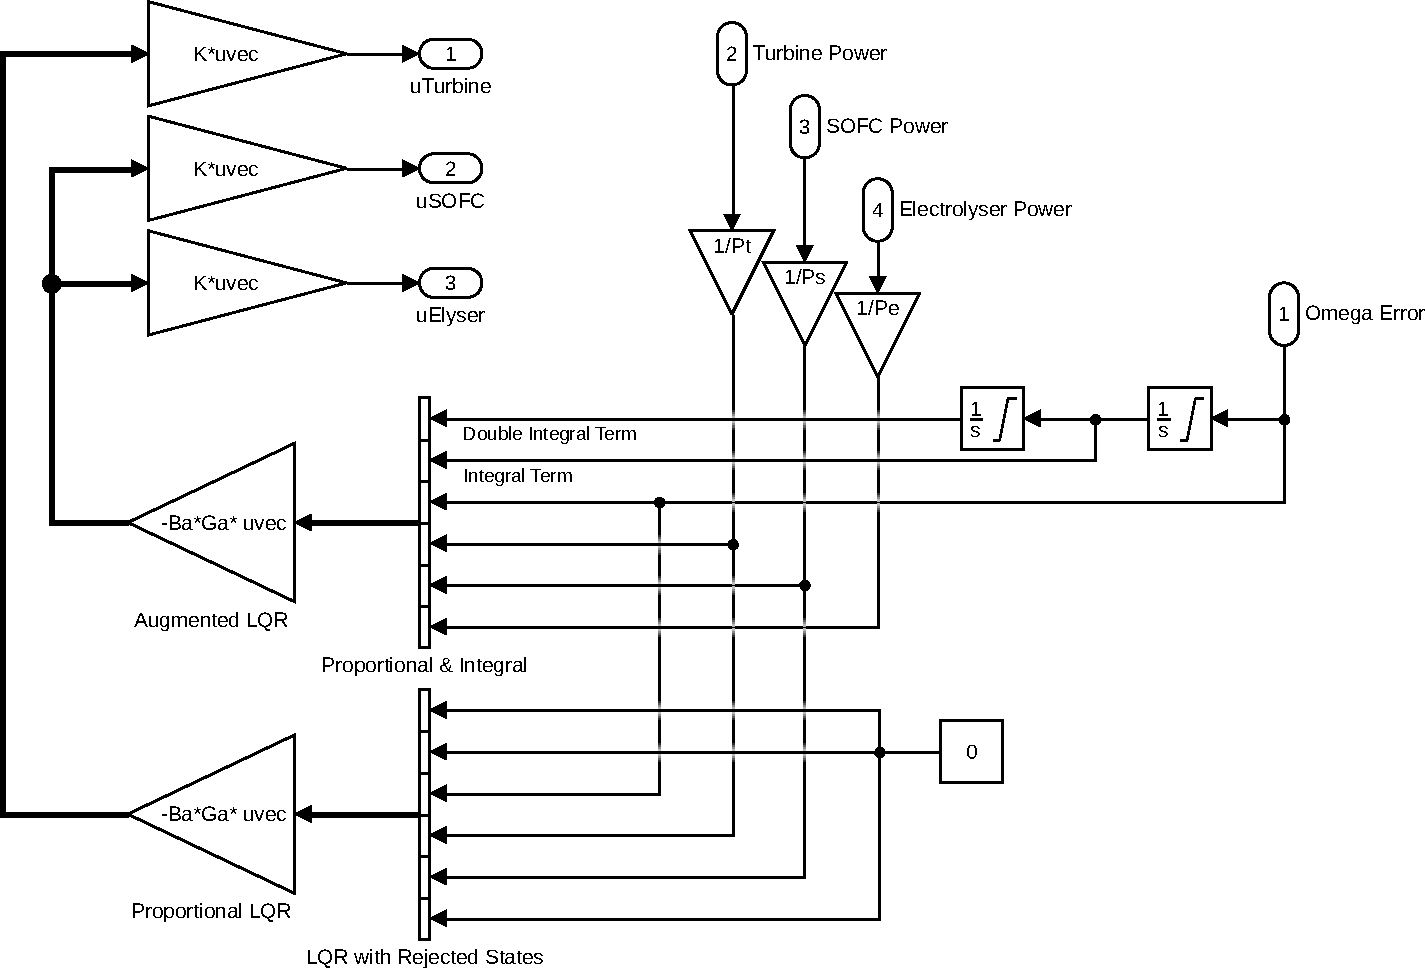
\includegraphics[scale=0.7]{images/plant2/ctrl.pdf}
    \caption{Controller Structure (LQR with Augmented State shown in Diagram)}
        \label{fig:ctrl}
\end{figure}
\begin{figure}[p]
\centering
        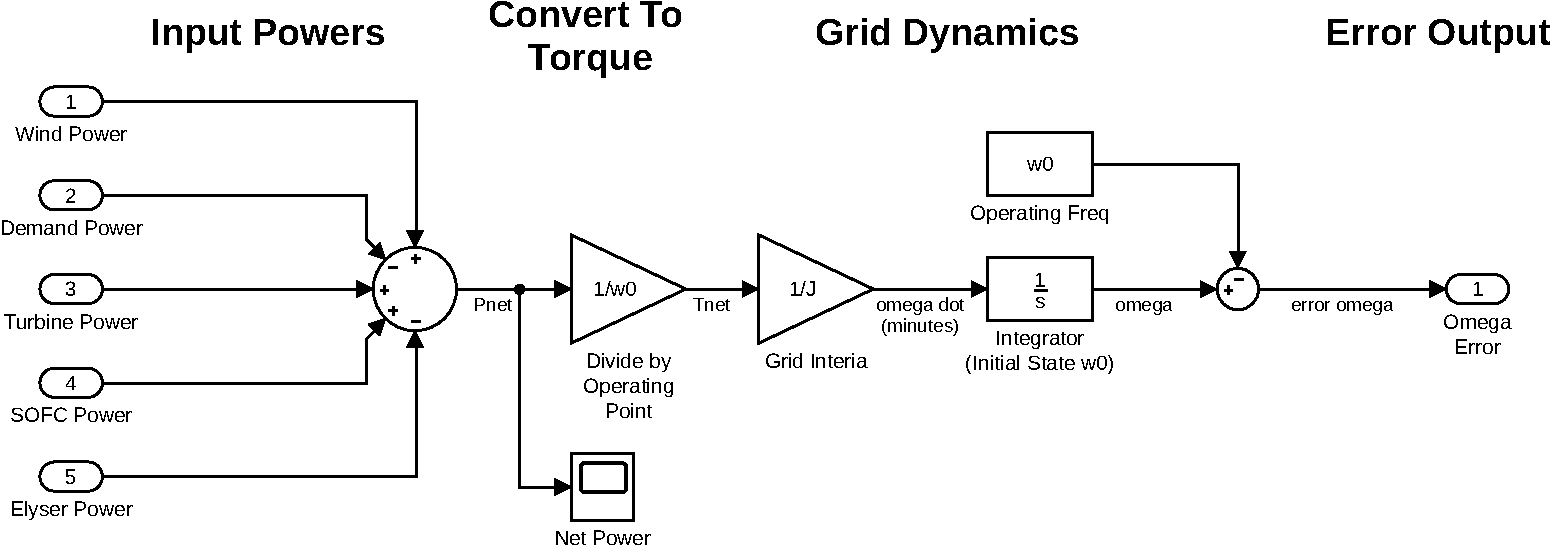
\includegraphics[scale=0.65]{images/plant2/grid.pdf}
    \caption{Grid Dynamics using Equation \ref{swing}.}
        \label{fig:grid}
\end{figure}
